% !TeX spellcheck = en_GB
\ifcsname SlidesDistr\endcsname%
\documentclass[handout,aspectratio=169]{beamer}
\else%
\documentclass[aspectratio=169]{beamer}
\fi%
\usepackage{fontspec}
\usepackage[T1]{fontenc}
\usepackage{amsmath}
\usepackage{amsfonts}
\usepackage{amssymb}
\usepackage{graphicx}
\usepackage{csquotes}
\usepackage{booktabs}
\usepackage{multicol}
\usepackage{enumerate}
\usepackage{microtype}
\usepackage[labelfont=bf,font={small}]{caption}
\usepackage{hyperref}
\usepackage{booktabs}
\usepackage{subcaption}
\usepackage{fancyhdr}
\usepackage{pdfpages}

\defaultfontfeatures{Mapping=tex-text}
\newfontfamily\symbolfont{Symbola}

\usepackage[sorting=none]{biblatex}
\addbibresource{../bibliography.bib}

\author{Andreas Stöckel}

\renewcommand{\vec}[1]{{\mathbf{#1}}}
\newcommand{\mat}[1]{{\mathbf{#1}}}

% Tango color palette
\definecolor{butter1}{HTML}{FCE94F}
\definecolor{butter2}{HTML}{EDD400}
\definecolor{butter3}{HTML}{C4A000}
\definecolor{orange1}{HTML}{FCAF3E}
\definecolor{orange2}{HTML}{F57900}
\definecolor{orange3}{HTML}{CE5C00}
\definecolor{chocolate1}{HTML}{E9B96E}
\definecolor{chocolate2}{HTML}{C17D11}
\definecolor{chocolate3}{HTML}{8F5902}
\definecolor{chameleon1}{HTML}{8AE234}
\definecolor{chameleon2}{HTML}{73D216}
\definecolor{chameleon3}{HTML}{4E9A06}
\definecolor{skyblue1}{HTML}{729FCF}
\definecolor{skyblue2}{HTML}{3465A4}
\definecolor{skyblue3}{HTML}{204A87}
\definecolor{plum1}{HTML}{AD7FA8}
\definecolor{plum2}{HTML}{75507B}
\definecolor{plum3}{HTML}{5C3566}
\definecolor{scarletred1}{HTML}{EF2929}
\definecolor{scarletred2}{HTML}{CC0000}
\definecolor{scarletred3}{HTML}{A40000}
\definecolor{aluminium1}{HTML}{EEEEEC}
\definecolor{aluminium2}{HTML}{D3D7CF}
\definecolor{aluminium3}{HTML}{BABDB6}
\definecolor{aluminium4}{HTML}{888A85}
\definecolor{aluminium5}{HTML}{555753}
\definecolor{aluminium6}{HTML}{2E3436}

\definecolor{violet}{HTML}{AA305C}
\definecolor{uwyellow}{HTML}{FDD433}
\definecolor{background}{HTML}{F9F9F6}
\definecolor{text}{HTML}{000000}

\definecolor{uweng1}{HTML}{D1B2EE}
\definecolor{uweng2}{HTML}{BF33DE}
\definecolor{uweng3}{HTML}{8001B3}
\definecolor{uweng4}{HTML}{56048A}

\setbeamercolor{title}{fg=violet}
\setbeamercolor{frametitle}{fg=black}
\setbeamercolor{structure}{fg=aluminium5}
\setbeamercolor{normal text}{fg=text}

\setbeamertemplate{navigation symbols}{}
\setbeamertemplate{footline}[frame number]


\newcommand{\hl}[1]{\colorbox{uwyellow}{{\textbf{#1}}}}

\newcommand{\ColorRect}[3]{{\color{#1}\rule{#2}{#3}}}
\setbeamertemplate{headline}{\ColorRect{black}{\textwidth}{4pt}\newline\ColorRect{uweng1}{0.25\textwidth}{4pt}\ColorRect{uweng2}{0.25\textwidth}{4pt}\ColorRect{uweng3}{0.25\textwidth}{4pt}\ColorRect{uweng4}{0.25\textwidth}{4pt}}

\newcommand{\MakeTitle}{
	\vspace{0.5cm}
	{\textbf{\inserttitle}}\\[0.5cm]
	\insertauthor\\[0.5cm]
	\insertdate\\
	\vspace{2cm}
 	\includegraphics[width=0.5\textwidth]{../assets/uwlogo_eng.pdf}
}

\newcommand{\handwritingframe}{%
	\begin{frame}
		\begin{columns}
			\column{\paperwidth}
			
\includegraphics{../assets/handwriting_lines.pdf}
		\end{columns}
	\end{frame}	
}


\date{February 4 \& 6 \& 11, 2020}
\title{SYDE 556/750 \\ Simulating Neurobiological Systems \\ Lecture 6: Recurrent Dynamics}

\begin{document}
	
	\begin{frame}{}
		\vspace{0.5cm}
		\begin{columns}[c]
			\column{0.6\textwidth}
			\MakeTitle
			\column{0.4\textwidth}
			\includegraphics[width=\textwidth]{media/canada_150_mosaic_engine_small.jpg}
		\end{columns}
	\end{frame}

	\begin{frame}{Feed Forward vs. Recurrent Connections}
		\centering
		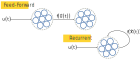
\includegraphics{media/feed_forward_recurrent.pdf}
	\end{frame}

	\begin{frame}{Recurrence Experiments (I)}
		\centering
		\includegraphics[width=\textwidth]{media/fxp1_example.pdf}
	\end{frame}

	\begin{frame}{Recurrence Experiments (II)}
		\centering
		\includegraphics[width=\textwidth]{media/fmx_example.pdf}
	\end{frame}

	\begin{frame}{Recurrence Experiments (III)}
		\centering
		\includegraphics[width=\textwidth]{media/fxs_example.pdf}
	\end{frame}

	\begin{frame}{NEF Principle 3: Dynamics}
		\begin{columns}[b]
			\column{0.5\textwidth}
				\centering
				\hl{Time-Invariant Dynamical System}\\
				\begin{align*}
					\frac{\mathrm{d}\vec x(t)}{\mathrm{d}t} &= f(\vec x(t), \vec u(t))
				\end{align*}
			\column{0.5\textwidth}
				\centering
				\hl{Linear Time-Invariant (LTI)}
				\hl{Dynamical System}
				\begin{align*}
					\frac{\mathrm{d}\vec x(t)}{\mathrm{d}t} &= \mat A \vec x + \mat B \vec u
				\end{align*}
		\end{columns}
		\vspace{0.75cm}
		\begin{mdframed}
			\textbf{NEF Principle 3 -- Dynamics}\\
			Neural dynamics are characterized by considering neural representations as control theoretic state variables. We can use control theory (and dynamical systems theory) to analyse and construct these systems.
		\end{mdframed}
	\end{frame}

	\begin{frame}{Making Sense of Dynamics}
		\centering
		\includegraphics[width=\textwidth]{media/synaptic_filter.pdf} 		
	\end{frame}

	\begin{frame}{Phase Portraits}
		\centering
		\includegraphics[width=\textwidth]{media/phase_portraits.pdf}
	\end{frame}

	\begin{frame}{Implementing Dynamics using a Neural Ensemble}
		\centering
		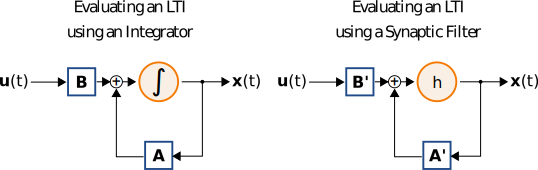
\includegraphics[width=\textwidth]{media/lti_integrator_vs_neural.pdf} 
	\end{frame}

	\begin{frame}{Implementing Dynamical Systems as a Neural Ensemble}
		\begin{columns}[t]
			\column{0.5\textwidth}
			\centering
			\hl{LTI System}
			\begin{align*}
				\phi(\vec u, \vec x) &= \mat A \vec x + \mat B \vec u \\
				\phi'(\vec u, \vec x) &= \mat A' \vec x + \mat B' \vec u \\
				\mat A' &= \tau \mat A + \mat I \\ \mat B' &= \tau \mat B \,.
			\end{align*}
			\column{0.5\textwidth}
			\centering
			\hl{Additive Time-Invariant System}
			\begin{align*}
				\phi(\vec u, \vec x) &= f(\vec x) + g(\vec u) \\
				\phi'(\vec u, \vec x) &= f'(\vec x) + g'(\vec u) \\
				f'(\vec x) &= \tau f(\vec x) + \vec x \\
				g'(\vec u) &= \tau g(\vec u)
			\end{align*}
		\end{columns}
		\vspace{1cm}
		\centering \hl{\enquote{General} Recipe}\\[0.25cm]
		Scale the original dynamics by $\tau$, add feedback $\vec x$
	\end{frame}

	\begin{frame}{Integrator Example (I)}
		\centering
		\includegraphics[width=\textwidth]{media/example_integrator.pdf}
	\end{frame}

	\begin{frame}{Integrator Example (II)}
		\centering
		\includegraphics[width=\textwidth]{media/example_integrator_phases.pdf}
	\end{frame}

	\begin{frame}{Oscillator Example (I)}
		\centering
		\includegraphics[width=\textwidth]{media/example_oscillator.pdf}
	\end{frame}

	\begin{frame}{Oscillator Example (II)}
		\centering
		\includegraphics[width=\textwidth]{media/example_oscillator_phases.pdf}
	\end{frame}

	\begin{frame}{Lorentz Attractor}
		\centering
		\includegraphics[width=\textwidth]{media/example_lorentz.pdf}
		\begin{align*}
			\frac{\mathrm{d}\vec x(t)}{\mathrm{d}t} &= \begin{pmatrix}
			10 x_2(t)-10x_1(t) \\
			-x_1(t) x_3(t)-x_2(t) \\
			x_1(t) x_2(t) - \frac{8}{3}(x_3(t)+28)-28
			\end{pmatrix}
		\end{align*}
	\end{frame}

	\begin{frame}{Heart Shape}
		\centering
		\includegraphics[width=\textwidth]{media/example_heart.pdf}
	\end{frame}

	\begin{frame}{Horizontal Eye Control}
		\centering
		\includegraphics[width=\textwidth]{media/example_eye_control.pdf}
	\end{frame}

	\begin{frame}{Administrative Remarks}
	\begin{itemize}
		\item \textbf{\hl{Project proposals}} due Friday, February 14\\ \url{http://compneuro.uwaterloo.ca/courses/syde-750/syde-556-possible-projects.html}\\[0.5cm]
		\item \textbf{\hl{Assignment 2}} due Thursday, February 13\\[0.5cm]
		\item \textbf{\hl{Assignment 3}} will be released later today, February 11 (due in three weeks)\\[0.5cm]
		\item Some adjustments to the schedule
	\end{itemize}
	\end{frame}


	\backupbegin

	\begin{frame}[noframenumbering]{Image sources}
		\small
		\textbf{Title slide}\\\enquote{The Canada 150 Mosaic Mural}\\Author: Mosaic Canada Murals.\\From \href{https://commons.wikimedia.org/wiki/File:Canada_150_Mosaic_Engine.jpg}{Wikimedia}.
	\end{frame}


	\backupend
	
\end{document}
